\section{Results}

\subsection{Showcase}
The following graphic shows a compilation of a running simulation in SUMO. The colors indicate the charge level of the vehicles and whether a vehicle is currently at a charging station and charging.

\begin{figure}[ht]
    \centering
    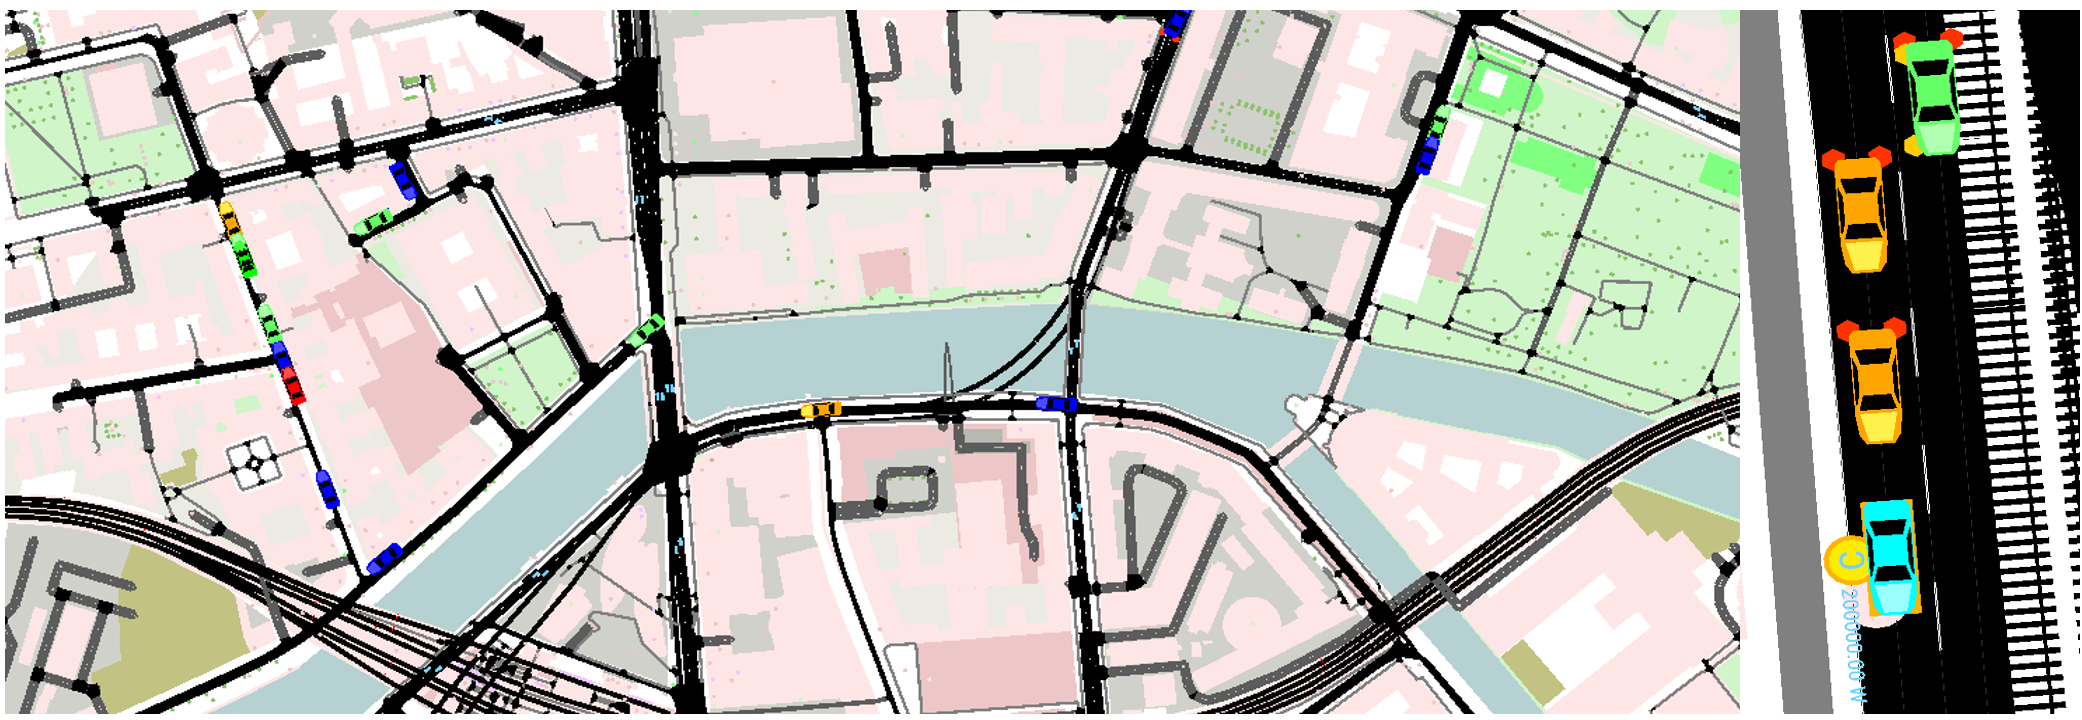
\includegraphics[width=\textwidth]{images/result_showcase.png}
    \caption{Showcase of current implementation}
    \label{fig:showcase}
\end{figure}

As described above, the charging stations were created as non-blocking lanes on the actual lanes. This means that vehicles charging there can charge without holding up the flow of traffic.

The vehicles drive to their POIs during rush hour. For example, in the morning they will drive to work between 7 and 9 a.m., stay there for an average of 8 hours, and then continue on to the next POI or back home. They follow their predefined routes.
TraCI reads the current charge level of the vehicles and colors them in the \texttt{sumo-gui} depending on their SoC. This facilitates qualitative evaluation.

If a vehicle's charge level falls below 20 percent of charge on its route, the implemented \texttt{stationfinder} ensures that the vehicle drives to the nearest charging station, where it is then charged. Once fully charged, the car then continues on to its originally intended POI.

\subsection{Functionalities}
The central functional modules of the first iteration that have already been implemented are listed and described in more detail below.

\newpage
\setlength\LTleft{-1cm}   % move 1cm left
\setlength\LTright{0pt}

\begin{longtable}{|
  >{\raggedright\arraybackslash}p{0.18\linewidth}|
  >{\raggedright\arraybackslash}p{0.38\linewidth}|
  >{\raggedright\arraybackslash}p{0.12\linewidth}|
  >{\raggedright\arraybackslash}p{0.16\linewidth}|
  >{\raggedright\arraybackslash}p{0.18\linewidth}|
}

\hline
\rowcolor{gray!20}
\textbf{Functionality} & \textbf{Description} & \textbf{Inputs} & \textbf{Outputs} & \textbf{Acceptance Criteria} \\
\hline
\endfirsthead

\hline
\rowcolor{gray!20}
\textbf{Functionality} & \textbf{Description} & \textbf{Inputs} & \textbf{Outputs} & \textbf{Acceptance Criteria} \\
\hline
\endhead

\hline
\multicolumn{5}{|r|}{\textit{Continued on next page}} \\
\hline
\endfoot

\hline
\endlastfoot

%%%%% OSM Import %%%%%
\rowcolor{gray!20}\multicolumn{5}{|l|}{\textbf{OSM Import}} \\
\hline
Selection \& download of OSM data
  & User selects a map area; system runs \texttt{osmGet} and saves the \texttt{.osm} file into the project directory.
  & Map selection
  & \texttt{.osm} file
  & \texttt{.osm} present in target folder
\\\hline
Convert OSM to SUMO network
  & Transforms the \texttt{.osm} file into a SUMO \texttt{network.xml} via \texttt{netconvert}.
  & \texttt{.osm} file
  & \texttt{network.xml}
  & Loads without errors in SUMO GUI
\\\hline

%%%%% Traffic Generation %%%%%
\rowcolor{gray!20}\multicolumn{5}{|l|}{\textbf{Traffic Generation}} \\
\hline
POI extraction
  & Parses \texttt{.osm}, filters by amenities (residential, commercial, school, etc.), and exports a geocoded CSV.
  & \texttt{.osm} file
  & \texttt{poi.csv}
  & POIs/amenities appear with valid lat/long entries
\\\hline
Trips generation
  & Generates \texttt{trips.xml} for N agents using map data and POI locations.
  & \texttt{.osm}, \texttt{poi.csv}
  & \texttt{trips.xml}
  & Agents assigned valid origin/destination
\\\hline
Automatic rerouting
  & Monitors vehicle SoC via TraCI and reroutes vehicles below threshold to nearest charger.
  & SoC threshold; charger list
  & Updated route assignments
  & Low-SoC vehicles rerouted within 30 s of threshold hit
\\\hline

%%%%% Charger Placement %%%%%
\rowcolor{gray!20}\multicolumn{5}{|l|}{\textbf{Charging Station Placement}} \\
\hline
Auto-place charging stations
  & Identifies lanes $\ge L_{\min}$ and assigns each a charger coordinate.
  & Minimum lane length $L_{\min}$
  & Charger coordinate list
  & 100\% of lanes $\ge L_{\min}$ receive one charger placement
\\\hline
Rank charging stations
  & In simulation, increment station score on each use; output a sorted list by usage frequency.
  & Simulation usage logs
  & Ranked station list
  & Ranked list of stations with number of all charge events
\\\hline
Iterative reduction of stations
  & Removes lowest-ranked chargers until only the top-K remain; outputs optimized placement.
  & Ranked station list
  & Optimized charger list
  & Top ranked stations are placed in simulation
\\\hline

%%%%% Simulation %%%%%
\rowcolor{gray!20}\multicolumn{5}{|l|}{\textbf{Simulation}} \\
\hline
Color vehicles by SoC
  & Via TraCI, color vehicles in GUI based on current SoC or charging status.
  & SoC thresholds; color mapping rules
  & Real-time colored visualization
  & Colored vehicles
\\\hline

%%%%% Performance %%%%%
\rowcolor{gray!20}\multicolumn{5}{|l|}{\textbf{Performance}} \\
\hline
Caching
  & Cache charger coordinates in memory to reduce repeated TraCI lookups and speed up simulation loops.
  & -- & -- & Simulator runtime reduced, no lags
\\\hline
\end{longtable}